
\section{Case study}
\label{sec:sysml}
To illustrate our approach, we take an example water tank as the case study inspired by \cite{AmalioPCW16}. According to the I/O dependency information between FMUs, the architectural model for water tank is constructed using SysML BDD, which helps to model the components and their connections.

%\subsection{Case Study: Water Tank}
The water tank system is shown in Fig.~\ref{tankfig}. A source of water flows into the water tank whose water flows into the drain. The source is controlled by a valve. When the valve is open, the water flows into the water tank. The valve, managed by a software controller, is opened or closed stochastically depending on the water level. In this paper, we illustrate three various version of water tank systems to show the scability of our approach. The difference between various water tank cases lies in various connection way between the controller, valve and tank. 
\begin{figure}[htbp]
	\centering	{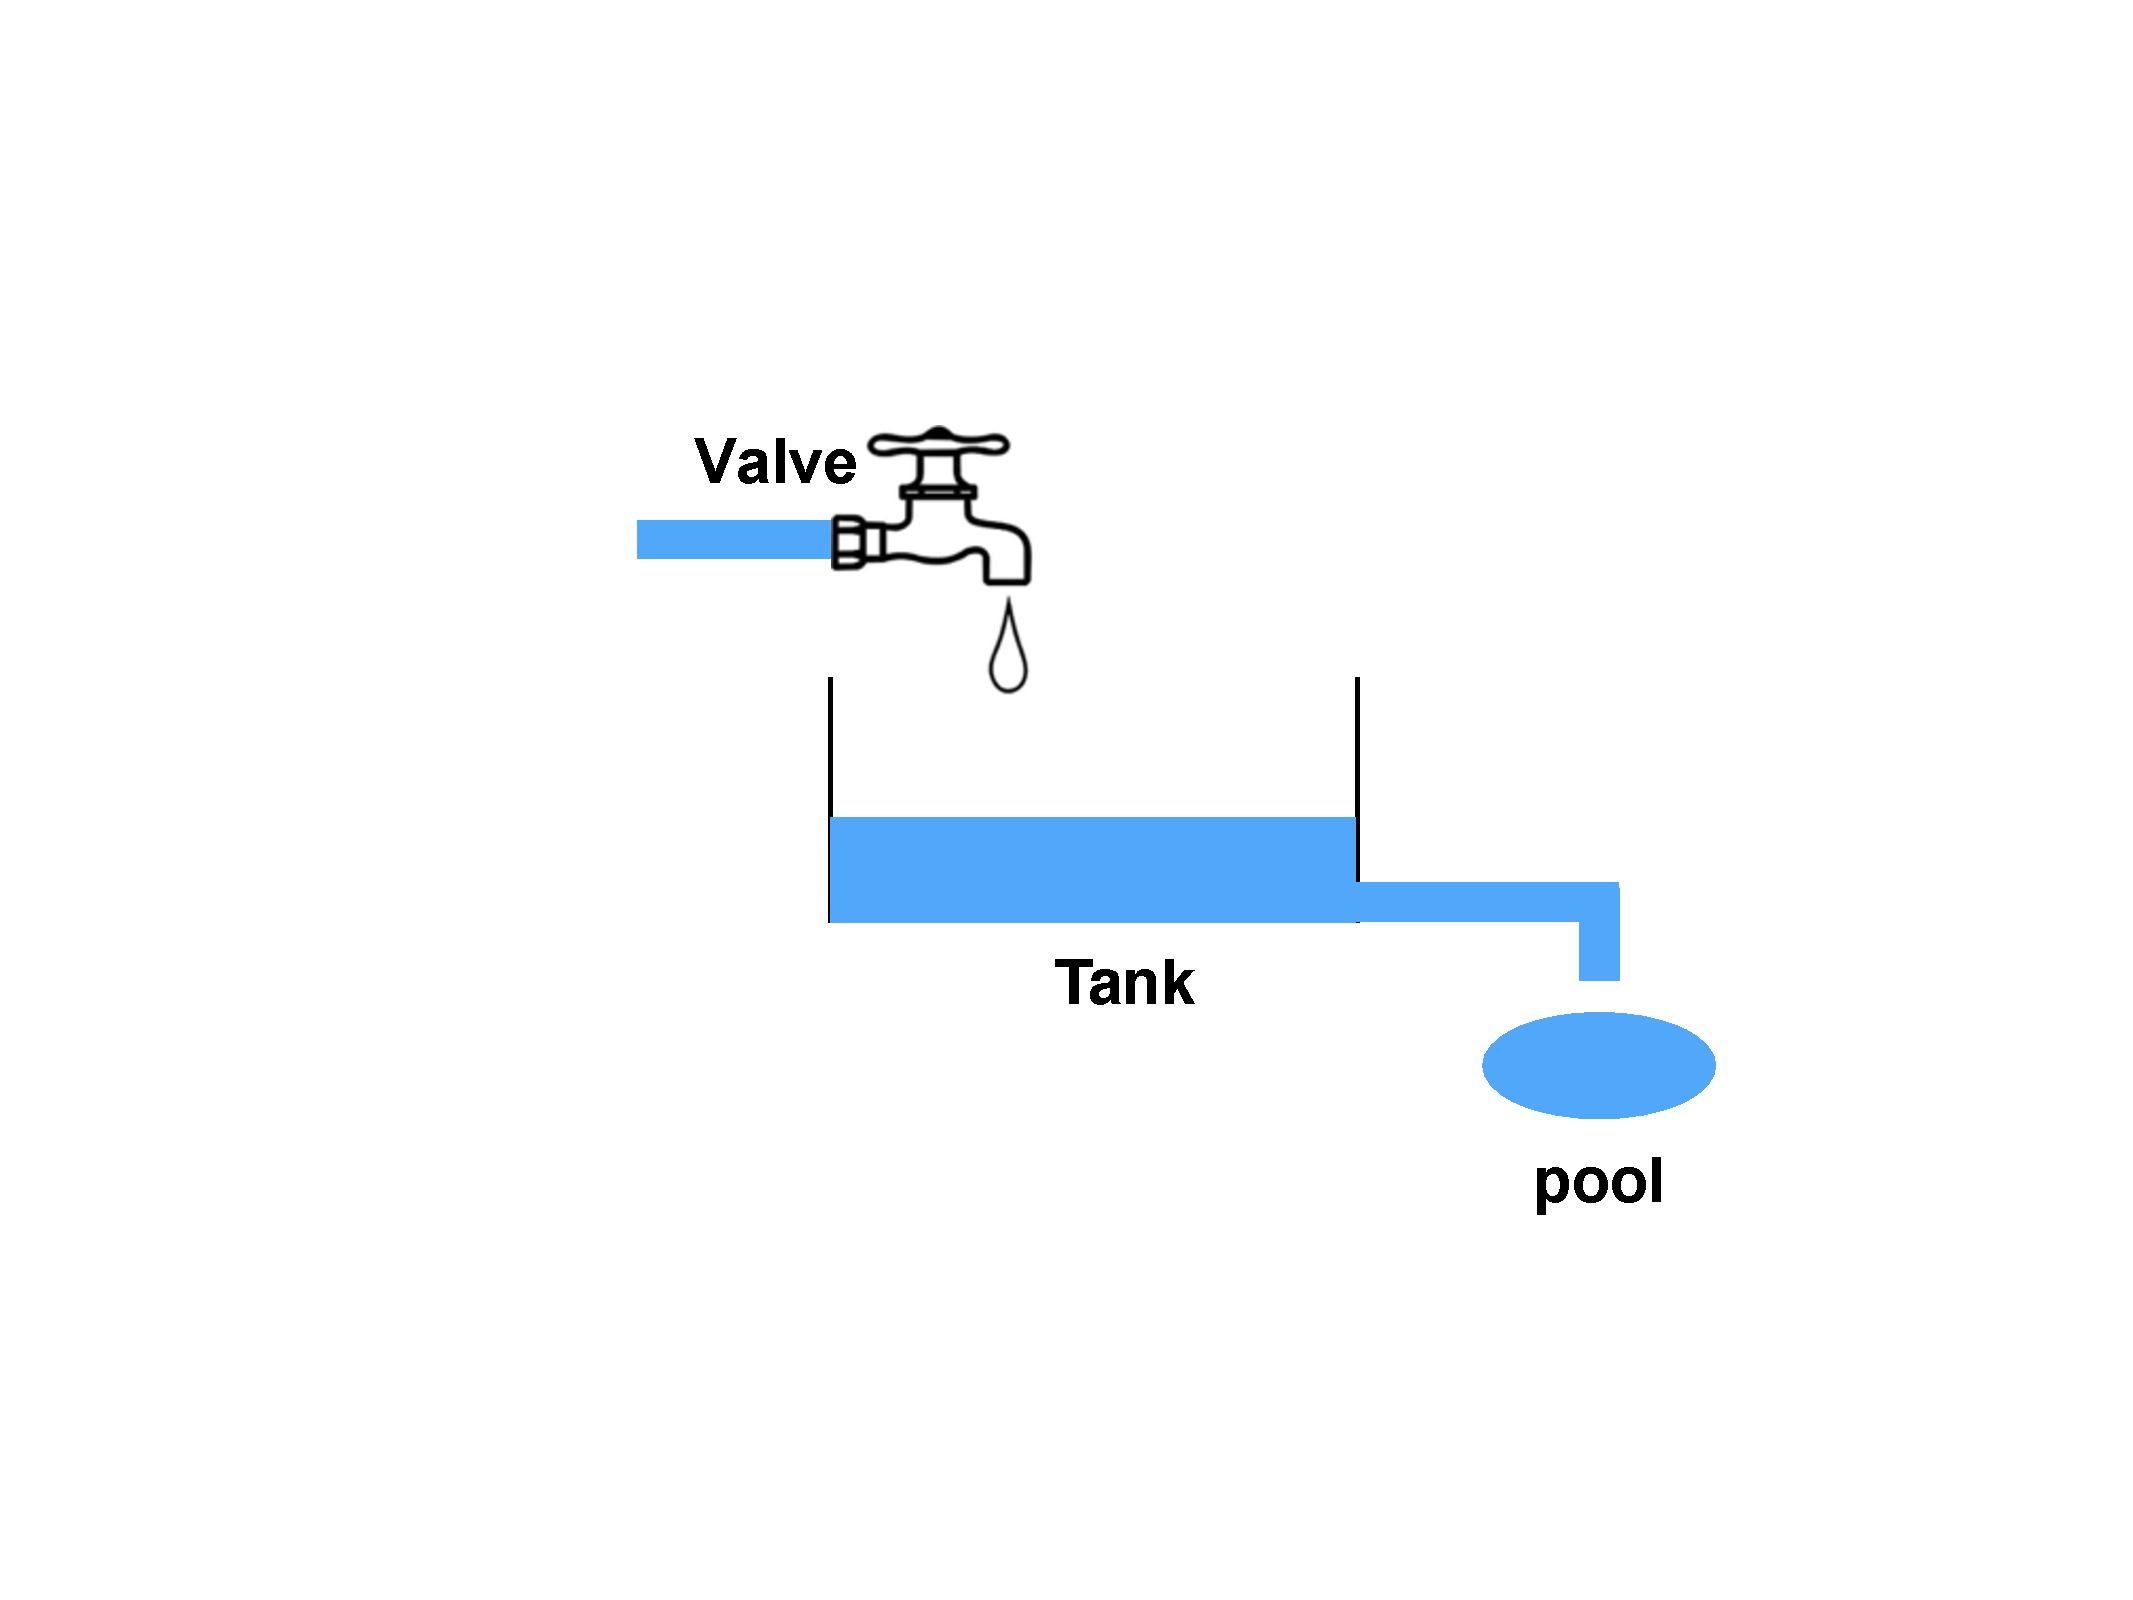
\includegraphics[width=1.7in,height=1.2in]{fig/tank-fig.pdf}}
	\caption{Water tank system.}
	\label{tankfig}
\end{figure} 
\subsection{Architecture Modeling with SysML}
SysML is a general purpose Domain-Specific Language (DSL) \cite{SemerathBHSV17} for Model-Based Systems Engineering (MBSE) \cite{Dori16}, which is originated as an initiative of the International Council on Systems Engineering (INCOSE) \cite{Pepper2015International} in January 2001. The SysML BDD describes the structure of the system with blocks. The IBD describes the internal structure and connections of blocks. The ports of blocks are connected by the connector. The I/O dependence of blocks describes the communication between blocks. SysML BDD is usually used to model the architecture of system.

Fig.~\ref{myad} shows the SysML BDD for the water tank system, which consists of three blocks: $Valve$, $Tank$ and $Controller$. $Valve$ and $Tank$ are physical components. $Controller$ is the cyber component. Each component has its own input and output. For instance, the input interface of $Valve$ is named as $vin$, which is used to input the $OpenClosed$ signal. 
\begin{figure}[htbp]
	\centering	{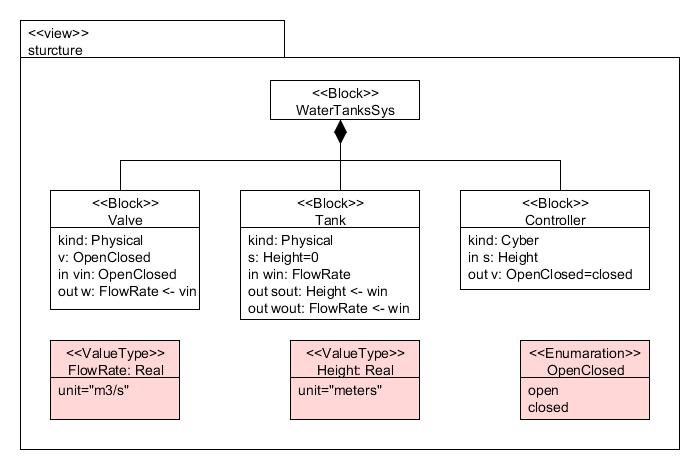
\includegraphics[width=3.2in,height=2.3in]{fig/AD.jpg}}
	\caption{SysML BDD for water tank.}
	\label{myad}
\end{figure}

Fig.~\ref{cd} shows the connection diagram for the system. There are three cases for connections. The first case is that the system has one valve, one controller and one tank. The controller sends stochastic signals to control the valve on/off leading to various rates of water flow. The second case is that the signal from the controller is affected by the water level of the tank. The last case is modified based on the first case and added another $waterTank2$ which is affected by the flow rate of the $waterTank1$.

\begin{figure}[htbp]
\centering{
		\subfigure[Connection case 1]{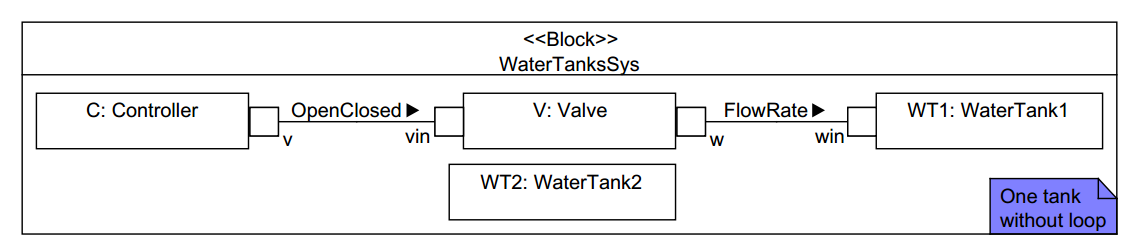
\includegraphics[width=3.2in,height=0.8in]{fig/CD1.png}
			\label{cd1}}
		\hfil
		\subfigure[Connection case 2]{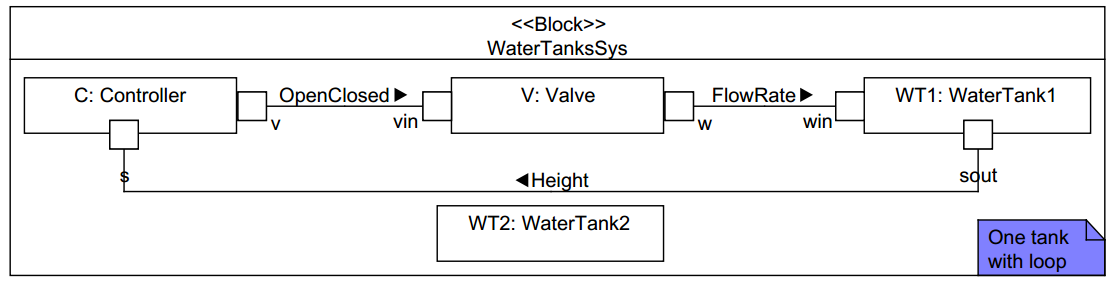
\includegraphics[width=3.2in,height=0.8in]{fig/CD2.png}
			\label{cd2}}
		\hfil
		\subfigure[Connection case 3]{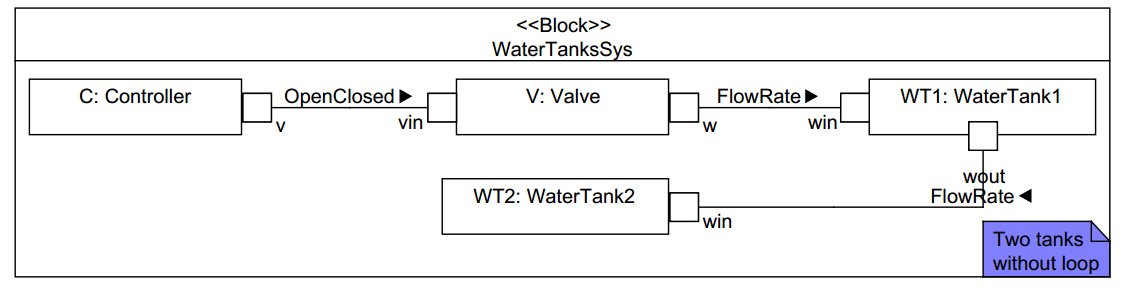
\includegraphics[width=3.2in,height=0.8in]{fig/CD3.png}
			\label{cd3}}
	\caption{SysML IBD for water tank.}
	\label{cd}
	}
\end{figure}
The SysML BDD shows the blocks of system and SysML IBD shows the connection between blocks. In next section, we abstract each block as an FMU, and model SysML IBD as the connector configuration.

\subsection{FMUs Connection of Water Tank}
Fig.~\ref{fmu-con} is the FMUs and FMUs connection of water tank system. There are three connection cases between the FMUs according to the SysML IBD shown in Fig.~\ref{cd}. The first case contains three FMU components $Controller$, $Valve$ and $WaterTank1$ and two channels $v \_ vin$, $w \_ win$ as shown in Fig.\ref{fmu-con1}. The $Controller$ and $Valve$ are connected with channel $v \_ vin$. The $Valve$ and $WaterTank1$ are connected with channel $w \_ win$. The second case is shown in Fig.\ref{fmu-con2}, there could be a channel $sout \_ s$ between $WaterTank1$ and $Controller$, which means the water level of $WaterTank1$ affects the control strategy of the \textbf{controller}. Fig.~\ref{fmu-con3} shows the third case, there could be another $WaterTank2$, the $WaterTank1$ and $WaterTank2$ are connected by the channel $w \_ out$. 
\begin{figure}[htbp]
\centering{
		\subfigure[Case 1]{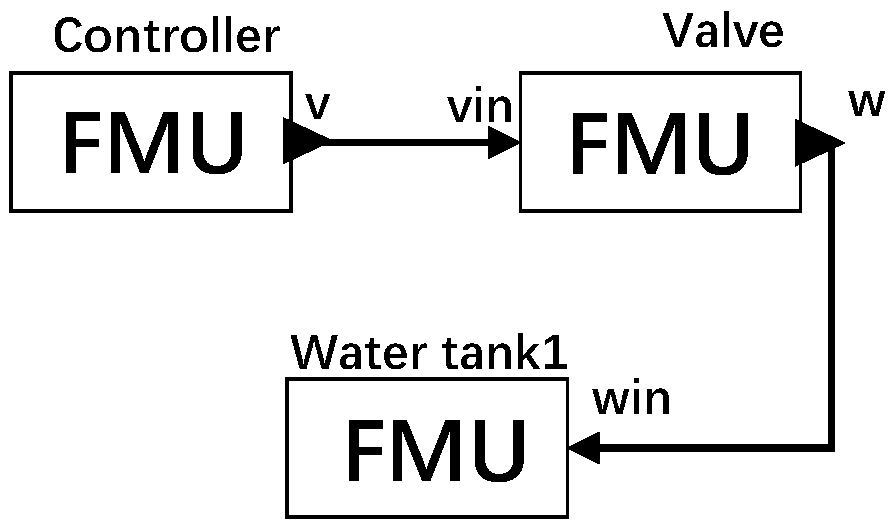
\includegraphics[width=1.0in,height=0.6in]{fig/fmuc1.png}
			\label{fmu-con1}}
		\hfil
		\subfigure[Case 2]{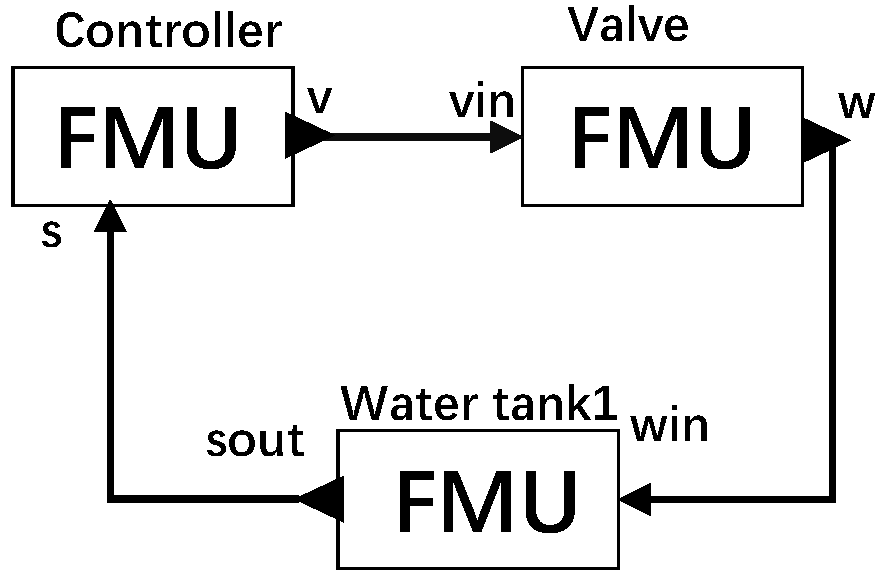
\includegraphics[width=1.0in,height=0.6in]{fig/fmuc2.png}
			\label{fmu-con2}}
		\hfil
		\subfigure[Case 3]{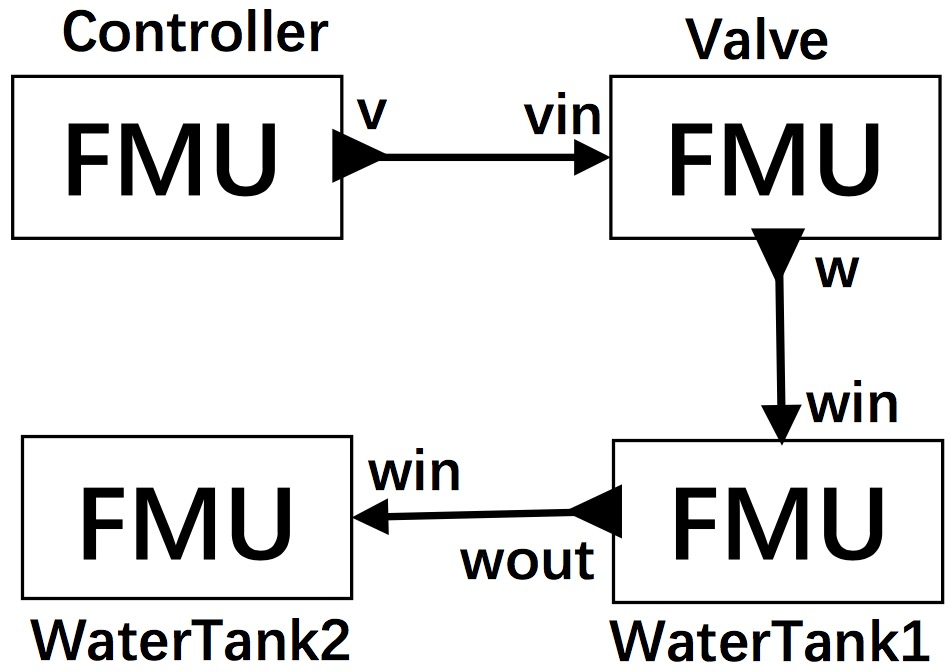
\includegraphics[width=1.0in,height=0.6in]{fig/fmuc3.png}
			\label{fmu-con3}}
	\caption{FMUs connections of three water tank cases.}
	\label{fmu-con}
	}
\end{figure}

Until now, we design the architecture and the connections of the case study. Before the system is co-simulated in the engine, how can we assure the correctness of the architecture models? To solve this problem, we use model checking to verify it. This is one of our main contributions. More details of verification process can be found in the next section.